\section{数値解析例}
本節では,Na型モンモリロナイトに対する水和エネルギーの式(\ref{eqn:del_G_mu})と
化学ポテンシャルの式(\ref{eqn:mu_system})を用いて行ったCG-MDシミュレーション
の結果を示す.シミュレーションでは,非平衡状態にあるNa型モンモリロナイト
含水系(以下,単に粘土含水系と呼ぶ)の初期モデルから,温度,相対湿度,
圧力を一定に保った緩和計算を行う.
これを6つの異なる相対湿度で行い,相対湿度に対する層間距離や粘土分子配置の
変化を調べる.以下では,初期モデルの作成を含めた計算手順について述べた後,
シミュレーション結果を示し,相対湿度に応じて組織構造にどのような差が現れる
かを述べる.
\subsection{初期モデル}
初期モデルを図\ref{fig:fig3}-(a)に示す.
これは2021年度の共同研究報告書で述べた方法で作成した
粘土含水系モデルの一つである.粘土含水系を構成する
分子数は80,粗視化粒子数は3,194で,
以下の計算を経て得られたものである.
はじめに,直線状の粘土分子を200$\times$200nm$^2$の矩形領域に,
互いに重ならないよう,位置と向きをランダムに配置する.
この矩形領域を周期構造の単位セルとして,乾燥密度が約1.6g/cm$^{3}$
となるまで断熱圧縮する.その際,粒子系の運動方程式を積分するための
時間ステップ幅は0.02ps,時間ステップ数は5万,
解析時間範囲は1nsとし,時間ステッピングに関する
条件は以後の解析でも同様である.断熱圧縮過程では,
系の温度を制御しないため,粘土含水系モデルは高い温度にあり,
平衡状態にも無い.そこで,圧縮後のモデルを300Kまで$250$psかけて冷却し,
その後750psにわたり温度を300Kに保って系を緩和する.
なお,ここでいう緩和とは,温度や体積などの外的条件を一定にして,
系を平衡状態へ推移させることを意味する.
以上の計算では,粗視化粒子が保持する水分量を表す粒子間相互作用ポテンシャルの
特性距離$\sigma$は,二層膨潤状態相当の$\sigma=1.5$nmに固定し,
系内での水分移動も系外との水分の授受も生じないものとしている.
最後に,無次元化された化学ポテンシャルを$\bar \mu =0.5$に保ち,
温度,体積一定のもと,水分移動を許容した
緩和計算を1ns間行う.このときの$\bar \mu$は強い排水が起こるように
設定されており,緩和計算後は比較的大きな層外空隙をもつ
組織構造が得られる.\\
\hspace{\parindent}
図\ref{fig:fig3}-(a)は,以上の方法で得られた粘土含水系モデルである.
本年度の研究では,これを初期構造とし,Na型モンモリロナイトの
水和エネルギーモデルを用いて,相対湿度一定で緩和計算を行う.
なお,初期構造を得る過程では,昨年度の研究で検討した
水和エネルギーモデルの一つである振動モデルを用いている.
このモデルは仮想的な粘土の水和挙動を表現したものであるため,
図\ref{fig:fig3}-(a)の状態は今回新たに作成した水和エネルギー
の下では平衡状態にない.そのため,緩和計算後には,
相対湿度の設定値によらず水分や分子配置には必ず何らかの変化が生じる.
%%%%
\subsection{相対湿度50$\%$に対する結果}
図\ref{fig:fig3}の(b)と(c)は,相対湿度50$\%$,温度300K, 圧力10MPaで
緩和計算を行ったときの粘土分子配置の変化を示したものである.
(b)は経過時間250psでの配置を,(c)は1ns経過して緩和計算を終了した
時点の結果を示している.この場合,初期状態(a)は水分量が少なく,
緩和計算初期の段階で速やかに吸水が起こる.その結果(b)では積層間隔が拡がり,
A$\sim$Dのラベルで示した層外間隙が(a)のときに比べて収縮する
一方,(b)から(c)の間には,粘土分子の配置にあまり大きな変化がなく,
(b)の時点から安定した構造が形成されていることがうかがわれる.
ただし,この間も間隙Aの収縮は進行し,(c)の段階ではほぼ消失している.
これに対して,粘土分子を巻き込むことで形成された層外間隙
CとDは,吸水に伴う収縮が比較的小さく,水分量の変化に対し組織構造
を維持する役割を果たしていると推察される.
なお,この計算では領域全体の体積は拘束されていないため,
状態(a)から(c)に移行する過程で,全体として若干の体積収縮が起きている.
このように,吸水による層間距離の拡張がある場合でも,
層外間隙の収縮が勝り,全体としては体積収縮がおきる可能性があることは,
マクロスコピックな膨潤挙動について議論する際にも留意すべき点と考えられる.
%--------------------
\begin{figure}[t]
	\begin{center}
	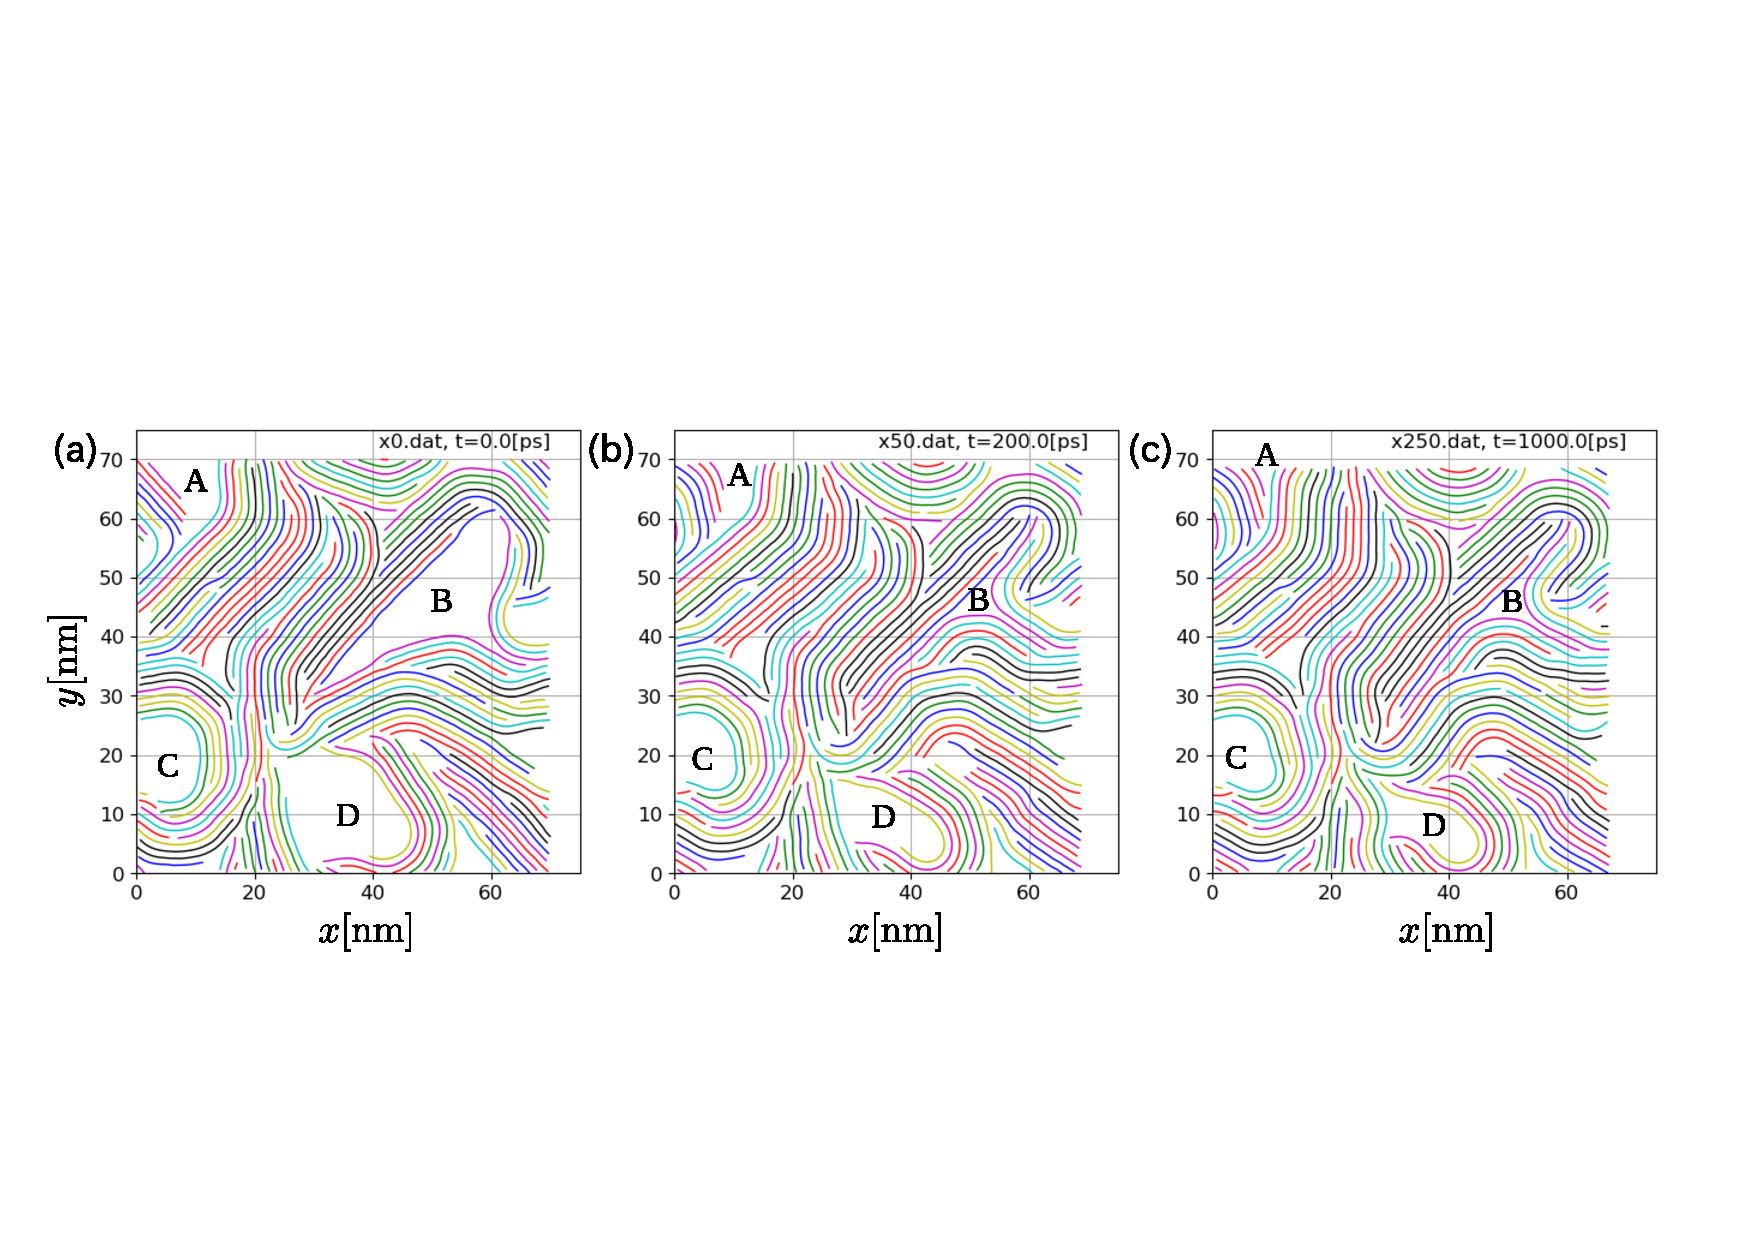
\includegraphics[width=1.0\linewidth]{Figs/fig3.pdf} 
	\end{center}
	\caption{
		相対湿度50$\%$での緩和にともなう粘土分子配置の変化.  
		(a)は初期状態,(b)緩和開始から200psの状態,(c)は1ns経過後の最終状態.
		A-Dのラベルは粘土層外の主要な間隙を示す.
	} 
	\label{fig:fig3}
\end{figure}
%--------------------
\begin{figure}
	\begin{center}
	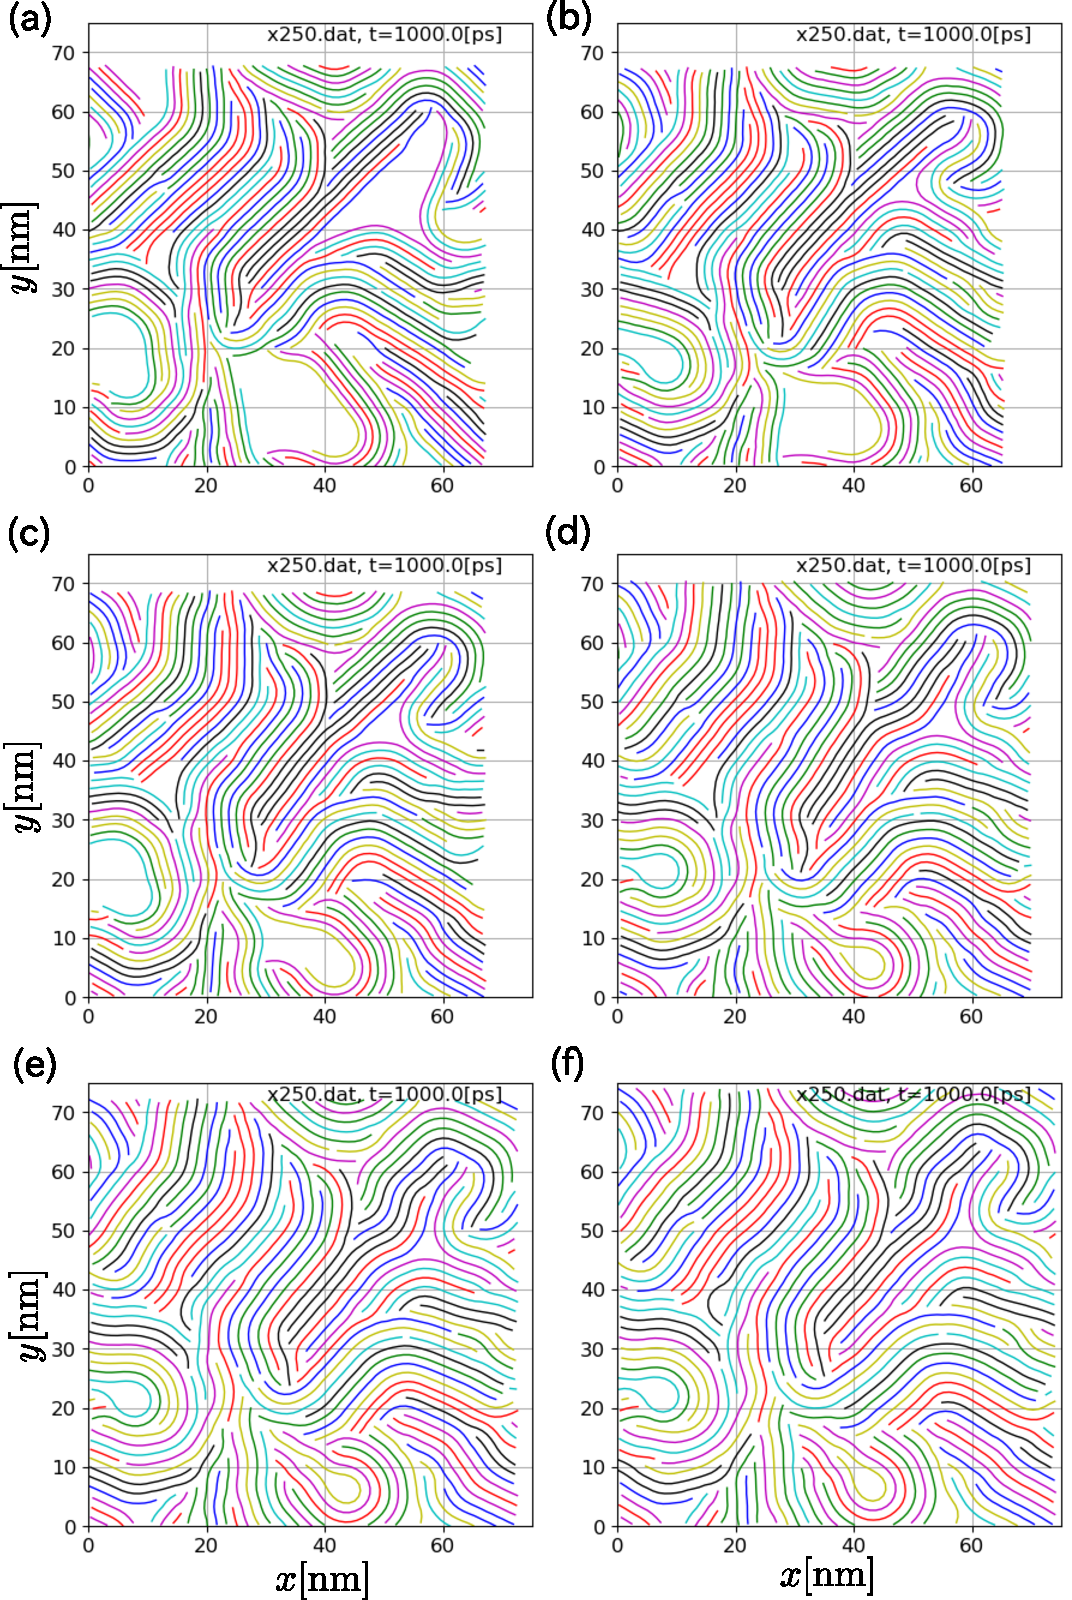
\includegraphics[width=0.8\linewidth]{Figs/fig4.pdf} 
	\end{center}
	\caption{
		6つの異なる相対湿度において得られた粘土含水系の組織構造.
		相対湿度は(a)から(f)の順に10,20,50,65,75および90$\%$. 
		相対湿度50$\%$の結果は,図\ref{fig:fig3}-(c)と同じものを再掲.
	} 
	\label{fig:fig4}
\end{figure}
\subsection{相対湿度による組織構造の違い}
ここまでに示した相対湿度50$\%$の場合に加え,相対湿度10,20,65,75および90$\%$
で緩和計算を行った結果を図\ref{fig:fig4}に示す.
図\ref{fig:fig4}の中で相対湿度が最も低い10$\%$の
ケース(a)では,初期構造(図\ref{fig:fig3}-(a))からあまり
変化がなく,層外間隙の形や大きさは当初と同程度に
とどまっている.これは,初期構造が,相対湿度$10\%$程度の
低い湿度で生じるものであったことを意味する.
ただし,系全体としては初期状態からやや収縮しており,
若干の排水が生じていると予想される.次に,2番目に
相対湿度が低い(b)20$\%$では,全体としては(a)と同程度の体積収縮
が生じている.一方で,層外間隙の一部は初期構造から大きく収縮する
ものがあり,分子配置は相対湿度50$\%$の結果(c)とよく似たものになっている.
ただし,相対湿度$50\%$のケース(c)と比べると,初期状態からみた
系全体の収縮量は(b)が大きく,(b)から(c)で次第に吸水膨張の効果が
大きくなっていることが読み取れる.
これに対して(d)65$\%$の場合,
全体としての体積変化はほぼ無視できる程度だが,
粘土の層間距離は(b)や(c)より大きくなっている.
そのため,吸水膨張の効果が系全体に及び,粘土分子の巻き込みで残留した
層外空隙もかなりの程度圧縮が進んでいる.さらに相対湿度の高い
(e)75$\%$と(f)90$\%$では,系全体としても膨張し始め,
このことは層外間隙の体積収縮が(d)から
大きく進行しないことと呼応している.\\
%--------------------
\begin{figure}
	\begin{center}
	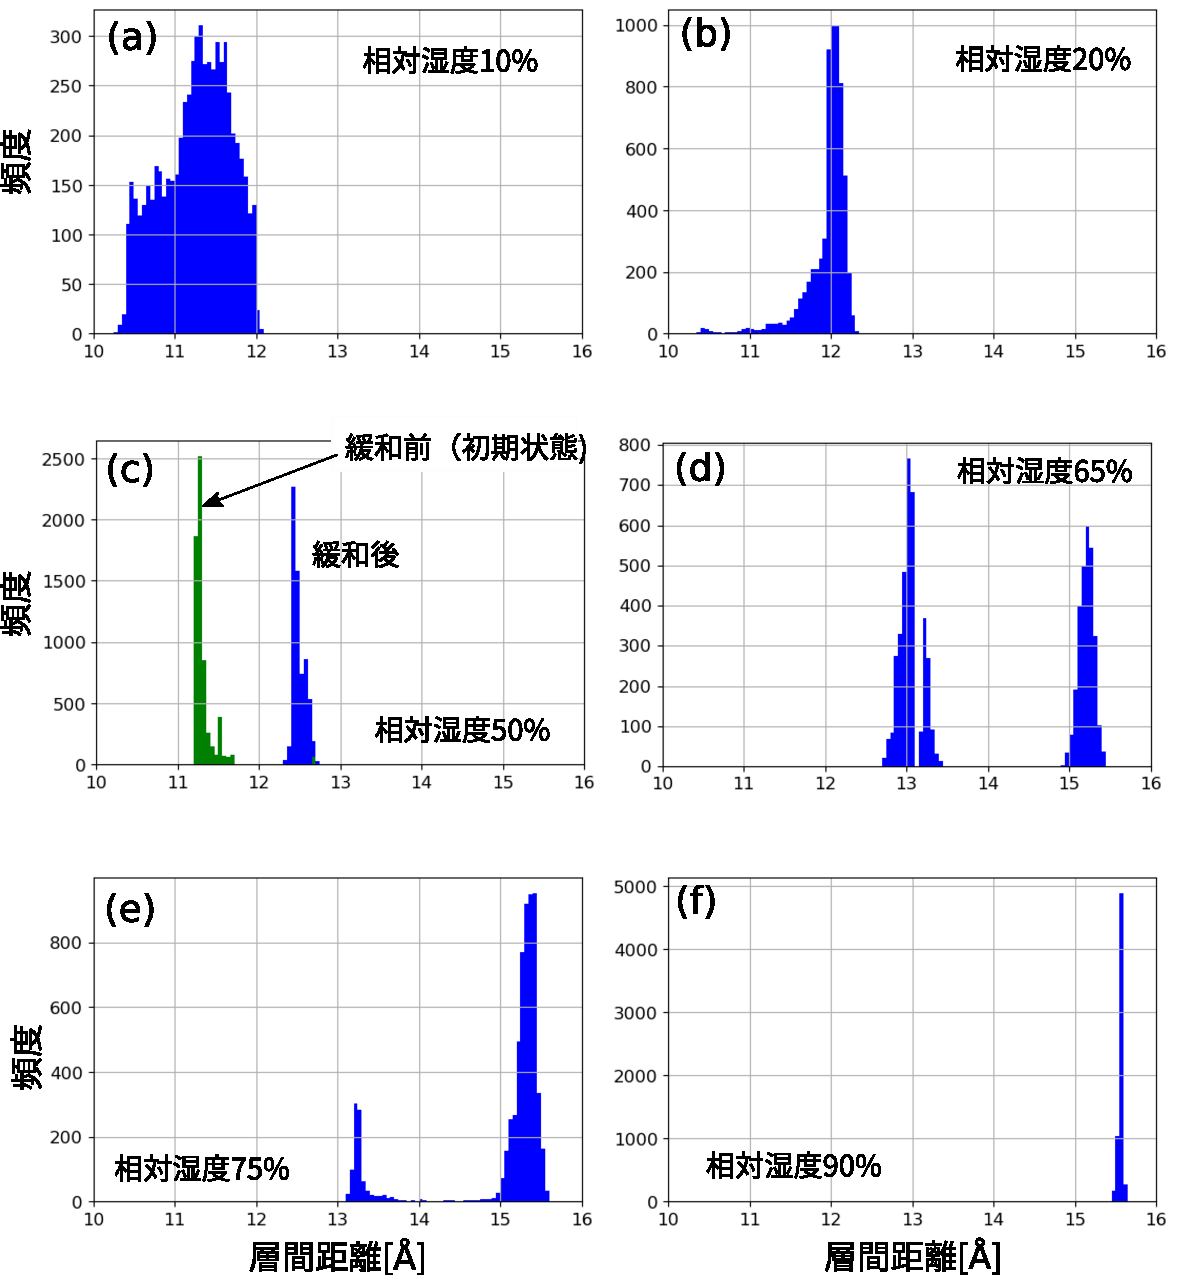
\includegraphics[width=1.0\linewidth]{Figs/fig5.pdf} 
	\end{center}
	\caption{
		6つの異なる相対湿度における層間距離の頻度分布.
		相対湿度は(a)から(f)の順に10,20,50,65,75および90$\%$. 
		(c)に示した緑の分布は,初期構造(緩和計算開始時)の
		層間距離の頻度分布を表す.
	} 
	\label{fig:fig5}
\end{figure}
%--------------------
\hspace{\parindent}
相対湿度と膨潤状態の関係を詳しく調べるために,相対湿度に対する層間距離の変化をみる.
図\ref{fig:fig5}は,そのために,層間距離の頻度分布を示したもので,
横軸が層間距離を,縦軸は頻度を表す. CG-MD法では,粒子間相互作用を与える
レナード-ジョーンズポテンシャルの特性距離$\sigma$で水分量を表現している.
$\sigma$は,概ね,粘土分子が積層したときの層間距離となるため,
$\sigma$を層間距離とみなし, その頻度分布を描いたのが図\ref{fig:fig5}である.
%横軸の範囲は,10から16$\AA$としており, 縦軸はグラフ毎に適切なサイズに描画されるように設定している.
%なお,図\ref{fig:fig1}-(a)にもあるように,系が気体状態の水
%に接している状態では,これらの頻度分布に示した範囲外の
%層間距離となることはない.
層間距離は,0膨潤で約10$\AA$,1および2層膨潤状態ではそれぞれ
約12.5$\AA$と15.5$\AA$である.ただし,図\ref{fig:fig1}-(a)からも分かるように,
天然のモンモリロナイトでは,0から2層の各膨潤状態に対応する層間距離を
厳密に定義することは難しく,上に挙げた層間距離は代表値と考えることが
より実情にあう.\\
\hspace{\parindent}
図\ref{fig:fig5}にあるように,層間距離は相対湿度の増加に伴いが
次第に大きくなり,頻度分布の峰は右方向へシフトする.
ただし,分布幅と形状は相対湿度毎に異なり,相対湿度が低いときと
複数のピークが現れる場合に分布幅が広くなる傾向がある.
また,個々の頻度分布に関しては以下のことが読み取れる.\\
\hspace{\parindent}
相対湿度が最も低い(a)では,他と比べて分布幅が明らかに広い.
このとき層間距離は10$\sim$12$\AA$の間にあり, 0層と1層膨潤の
中間的な状態になっている.次に相対湿度の低い(b)では,層間距離が
12$\AA$周辺に集中し,ほぼ1層膨潤状態に移行していることが分かる.
ここで,図\ref{fig:fig1}-(a)の粉末X線回折試験結果を見ると,
相対湿度10$\sim$20$\%$での層間距離は約10$\AA$で0層膨潤となっている.
従って,CG-MD計算の方が,同じ湿度でより多くの水分が保持される
結果となっている. これは,(a)の状態から更に排水を進めるには
粘土分子の積層構造を変化させる必要があり,そのためには,同程度の
水分をもつ粉末状態の粘土から脱水するよりも多くのエネルギーが
必要とされることを意味している.\\
%逆に言えば,指定された初期構造から0層膨潤状態に移行させるためには,
%より大きなエネルギーを加えて計全体を強く圧縮するか,組織構造
%を破壊する必要があることを示唆している.
\hspace{\parindent}
次に,相対湿度50$\%$の結果(c)を見ると,分布幅が狭く層間距離はほぼ
12.5$\AA$と,粉末X線回折試験結果とよく一致している.
%また,相対湿度$50\%$では,系全体としての体積変化膨張を起こすことなく水分が
%取り込まれていることから,初期構造から到達および維持されやすい組織構造に
%なっていると考えられる.
続いて(d)65$\%$と(e)75$\%$の結果を見ると,3つあるいは2つピークをもつ
多峰分布となっている.粉末X線回折試験結果(図\ref{fig:fig1}-(a))を参照すると,
これらの相対湿度は1層から2膨潤への遷移領域にあることが分かる.
従って,13$\AA$と15.5$\AA$付近のピークは,それぞれ,1層および2層膨潤
に対応し,2つの膨潤状態が混在していると判断できる.
一方,14$\AA$付近の層間距離は現れず,このことは,1層と2層の中間的状態
を経ることなく膨潤状態が推移する,Na型モンモリロナイト特徴的な挙動が
CG-MDシミュレーションに反映されていることを意味する.
%
ここで,(d)の結果をより細かく見ると,13$\AA$前後で大小2つのピークが存在する.
このうち大ピークは安定な1層膨潤状態にとどまっている層間水を,
小ピークは既に2層膨潤へ移行を開始しつつあるものの,十分な水分が
なく1層膨潤付近にとどまる層間水の存在を示している.
これら大,小ピークの谷にあたる13.1$\AA$では,図\ref{fig:fig1}-(a)の
膨潤曲線が大きく折れ曲がり,この層間距離を境に膨潤挙動が変化している.
この点を踏まえれば,(d)より相対湿度がやや高い(e)において大ピークが消失する
ことは,(e)は全ての層間水が2層膨潤状態に向けて移行を開始した状態にあると
解釈できる.最後に,最も相対湿度の高い(f)では,2層膨潤への移行が完全に終了し,
鋭いピークを持つ層間距離分布となっている.このときピーク位置は15.5$\AA$で,
粉末X線回折試験結果で観察される層間距離とよく一致している.\\
\hspace{\parindent}
%なお,(d)に見られる第3の小ピークを伴う遷移挙動が実際の固体粘土で観察も
%現れるのか,
以上のように,1層から2層膨潤状態への推移に関しては,
Na型モンモリロナイトの粉末X線回折試験結果に見られる
離散的な層間距離の変化がよく現れている.
一方,相対湿度の低いケースでは
0層膨潤状態が明確に現れず,1層から0層膨潤への移行が粘土分子の
積層構造に妨げられる結果となった.
このような挙動が実際の粘土でも現れるのか,またその影響がX線回折パターン
にも反映されるかは,メソスケール組織構造を実験的に調べる上で
興味深い問題の一つになると思われる.
